\documentclass[11pt]{article}
\usepackage[margin=1in]{geometry}
\usepackage{amsmath}
\usepackage{graphicx}
\usepackage{booktabs}
\usepackage{epigraph}
\usepackage{authblk}
\usepackage[hidelinks]{hyperref}
\setlength{\epigraphwidth}{0.72\textwidth}

\title{\textbf{Cartesian similarity is a poor proxy for transition-state
quality: reference databases penalize valid alternative saddles}}
\author[1,3]{Kfir Kaplan\thanks{kfir.k4@gmail.com}}
\author[1,2,3]{Alon Grinberg Dana}
\affil[1]{Wolfson Department of Chemical Engineering, Technion -- Israel Institute of Technology, Haifa 3200003, Israel}
\affil[2]{Grand Technion Energy Program (GTEP), Technion -- Israel Institute of Technology, Haifa 3200003, Israel}
\affil[3]{Boeing-Technion SAF Innovation Center, Technion -- Israel Institute of Technology, Haifa 3200003, Israel}
\date{\today}

\begin{document}
\maketitle

\begin{abstract}
Machine-learning models for transition-state (TS) geometry prediction are almost
universally benchmarked by the root-mean-square deviation (RMSD) of atomic
positions, or by the mean absolute error of the interatomic-distance matrix
(D-MAE), relative to a reference transition state. Both are Euclidean similarity
measures. We show that they are poor proxies for the quantity that actually
matters to a practitioner: whether a predicted geometry optimizes to a genuine
transition state at a target level of density functional theory (DFT). Optimizing
$520$ interpolation-based guesses for $260$ reactions from the Transition1x
database at the r$^2$SCAN-3c level, we find that \emph{every} geometry-based
quality measure - Kabsch-aligned RMSD, D-MAE, a reaction-coordinate projection,
and cheap semi-empirical descriptors - saturates in a narrow band of the area
under the receiver-operating-characteristic curve (AUC; defined in
Section~\ref{sec:metrics}), $0.77$--$0.84$, for predicting optimization success,
with about $14\%$ of low-RMSD guesses nonetheless failing. Decomposing
the ``failures'', $38\%$ converge to a genuine but \emph{different} first-order
saddle point (median energy difference $1.36$~eV from the reference, $77\%$ of
them \emph{lower} in energy); these are legitimate alternative transition states
that a reference-matching metric penalizes as errors. Only about $13\%$ are
symmetry-equivalent artifacts, which we remove algorithmically. Once RMSD is held
fixed, no structural property of the reactant or product distinguishes converging
from failing guesses: convergence is governed by the topology of the
potential-energy surface (PES) - competing saddles and basins - which a
Cartesian distance cannot see. A controlled experiment identifies the cause.
Displacing each reference saddle by a \emph{prescribed} distance along different
directions - the reaction mode, the softest and stiffest vibrations, and
isotropic noise - changes the probability of recovering it from $33\%$ to $98\%$
at identical distance, so distance alone cannot determine the outcome; yet once
direction is held fixed as well, the ceiling persists at AUC $\approx 0.83$. The
saturation is therefore a limit on what a guess geometry can express, not a
defect of any particular metric. All conclusions replicate on a second,
chemically broader database covering second- and third-row elements, on which
discrimination at matched guess quality is no better than on Transition1x, and on
a state-of-the-art flow-matching generator: oracle best-of-$N$ selection roughly
triples its deployable single-draw success rate, yet no reference-free score
recovers that gain, so reported best-of-$N$ figures overstate what a user obtains
by about threefold.
We conclude that (i)~the saturation near AUC $0.84$ is an information ceiling
rather than a shortcoming of any metric: a guess geometry simply does not encode
how large the basin around its target saddle is, and the best geometric measure
we construct already operates at that limit; (ii)~RMSD and D-MAE compound this by
measuring similarity to one arbitrarily chosen saddle rather than usefulness,
while reference databases such as Transition1x are energetically skewed, so
interpolation guesses routinely locate \emph{lower-energy} saddles absent from
the reference - whether these are alternative, stepwise, or unrelated transition
states is, for these open-shell systems, beyond the reach of current automated
structure perception (itself a cautionary result); and (iii)~as a practical
consequence, a cheap GFN2-xTB force descriptor evaluated on the guess predicts
convergence about as well as oracle RMSD while requiring no reference structure -
useful precisely because the ceiling means nothing better is available.
\end{abstract}

\section{Introduction}

Predicting transition-state (TS) geometries is a central problem in computational
reaction chemistry, and a rapidly growing set of machine-learning models now
addresses it --- from the early graph-based generator TS-GCN~\cite{TSGCN} through
diffusion models that build the saddle from a 2D graph~\cite{TSDiff} or from 3D
reactant and product structures~\cite{Duan2023}, to the recent optimal-transport
and flow-matching approaches~\cite{ReactOT,GoFlow,RitS}. These are trained largely
on the Transition1x database~\cite{Schreiner2022} and evaluated on held-out
reactions from it. Almost without
exception these models are evaluated by geometric similarity to a reference
transition state - the root-mean-square deviation (RMSD) of atomic coordinates
after optimal superposition, or the mean absolute error of the
interatomic-distance matrix (D-MAE).

The reason the field defaults to these Cartesian measures is practical rather
than principled: the physically correct test of a predicted transition state -
optimizing it to a first-order saddle and verifying, via an intrinsic reaction
coordinate (IRC)~\cite{Fukui1981}, that it connects the intended reactant and
product - requires Hessians and reaction-path integrations that are far too
expensive to run for every prediction during model development. Machine-learned
Hessians~\cite{Yuan2024} and reactive interatomic potentials~\cite{Busk2023}
lower this cost but do not remove the need for a target-level verification. A
cheap geometric distance to a stored reference is an attractive surrogate. Implicit in its use is
an assumption that, to our knowledge, has never been tested directly: that a lower
similarity to the reference implies a more \emph{useful} guess, i.e.\ one more
likely to converge, under a standard saddle-point optimizer, to a valid
transition state.

We test that assumption. We take deliberately simple, geometry-only predictors,
optimize their guesses at a consistent density-functional-theory (DFT) level, and
ask what - if anything - about a guess predicts whether it converges. The
answer is sobering, and it points less at the models than at the way we benchmark
them and at the reference data itself.

Our findings are the following. (1)~Every geometric measure of guess quality we
test saturates in a narrow band of predictive power, area under the
receiver-operating-characteristic curve $0.77$--$0.84$, and a purpose-built
motion-weighted measure sits at the top of it. (2)~A controlled experiment, in
which reference saddles are displaced by a fixed distance along chosen normal
modes, shows this is not a defect of the measures but an information ceiling: at
identical distance the outcome swings from $33\%$ to $98\%$ with the
\emph{direction} of displacement, and even with direction fixed the ceiling
persists --- because reactions differ irreducibly in the size of the basin around
their saddle, which no guess geometry encodes. (3)~A large share of apparent
failures are not failures but genuine, often lower-energy, alternative saddles
that a reference-matching metric penalizes, exposing an energetic skew in the
reference database. (4)~The conclusions hold on a second, chemically broader
database and, most consequentially, for a state-of-the-art generative model:
oracle best-of-$N$ selection roughly triples its deployable success rate, but no
reference-free score recovers that gain, so reported best-of-$N$ figures overstate
what a user obtains. Throughout, we avoid drawing conclusions from quantities a
practitioner cannot compute without already knowing the answer.

\section{Methods}

\subsection{Data and reference}
We use the Transition1x database~\cite{Schreiner2022} of reactant, product and
transition-state geometries (originally at the $\omega$B97x/6-31G(d) level). To
obtain an internally consistent reference at our working level, we re-optimize
each Transition1x transition state at the r$^2$SCAN-3c composite DFT
level~\cite{Grimme2021} (ORCA~6.0.0~\cite{Neese2025}). The set comprises $260$
reactions ($520$ guesses); $259/260$ reference saddles converge, all with exactly
one imaginary vibrational frequency, confirming genuine first-order saddle points.
Reactants and products are likewise optimized at r$^2$SCAN-3c to
define the minima used for connectivity. Areas under the curve
(Tables~\ref{tab:weights} and~\ref{tab:auc}, Figure~\ref{fig:ceiling}) are reported
on the $200$-reaction batch ($400$ guesses) for which the complete descriptor set,
including the GFN2-xTB features, was computed; the alternative-saddle census
(Section~\ref{sec:alt}) uses all $260$ reactions ($520$ guesses).

To test generalization beyond first-row organic chemistry, we repeat the whole
protocol on a second database, Reaction-QM~\cite{ReactionQM2026}. We use only its
density-functional-optimized subset (B3LYP-D3/TZVP), from which we sample $200$
unimolecular reactions; these contain second- and third-row elements absent from
Transition1x. All geometries are re-optimized at r$^2$SCAN-3c exactly as above, so
the two databases are compared at an identical working level and under an
identical success criterion. Results are reported in Section~\ref{sec:rqm}.

\subsection{Predictors}
Two geometry-only predictors generate the guesses whose fate we study:
\emph{midpoint}, the linear interpolation $\tfrac{1}{2}(D^{R}+D^{P})$ of the
reactant and product distance matrices, embedded in three dimensions by classical
multidimensional scaling (MDS); and \emph{bond-order}, which models the length of
each reactive bond from Pauling's bond-order/bond-length relation and interpolates
the remaining pairs. These are not intended to be competitive with modern
learned models; they are cheap, transparent sources of realistic guesses.

\subsection{Downstream optimization and success}
From each guess we run a transition-state optimization with analytic Hessians
(ORCA \texttt{OptTS}) followed by a vibrational analysis. A guess is counted a
\emph{success} if the optimization converges, the result has exactly one
imaginary frequency, and its Kabsch-aligned RMSD to the reference saddle is below
$0.3$~\AA. Optimization cost is recorded as the number of geometry cycles and the
wall-clock time.

\subsection{Metrics and their evaluation}
\label{sec:metrics}
We compare guess-quality measures both requiring the reference TS (Kabsch RMSD;
D-MAE; a change-weighted D-MAE; a projection of the aligned error onto the
reaction coordinate, split into components parallel and perpendicular to it; the
un-normalized root-square deviation; and a reactive-atom-only RMSD) and
\emph{deployable} descriptors requiring only the guess and the reactant/product
(the GFN2-xTB force norm on the guess, and its energy relative to the endpoints).
GFN2-xTB~\cite{Bannwarth2019} denotes the second-generation geometry-, frequency- and non-covalent-
interaction-parametrised semi-empirical tight-binding method.

Because the outcome is binary (success or failure), we quantify how well a
continuous measure separates the two classes by the area under the
receiver-operating-characteristic curve, abbreviated AUC. The
receiver-operating-characteristic curve plots the true-positive against the
false-positive rate as a decision threshold is swept; its area equals the
probability that a randomly chosen failure is assigned a larger error than a
randomly chosen success. An AUC of $0.5$ is uninformative (a coin flip) and $1.0$
is perfect separation; the measure is threshold-free and invariant to monotone
rescaling.

\subsection{Controlled displacement experiment}
To test whether the saturation of the metrics is a property of the metrics or of
the surface, we construct guesses whose deviation is fixed by design rather than
observed. Each reference saddle is relaxed to a GFN2-xTB~\cite{Bannwarth2019}
saddle with the Sella optimizer, and the Hessian is computed there by finite
differences. Displacement directions are taken as the imaginary mode, the softest
and stiffest internal vibrations, and an isotropic Gaussian vector. Because
Kabsch alignment removes rigid-body motion, the six translation/rotation modes are
projected out of every direction before use --- without this, a mode dominated by
rotation produces a displacement an order of magnitude smaller than its nominal
length. The step length is then solved by bisection so that the achieved Kabsch
RMSD equals the target; the achieved value is stored for every trial and checked
during analysis. The saddle search is repeated from each displaced structure and
counted as a return if it converges within $0.3$~\AA\ of the original xTB saddle.
This uses $187$ (Transition1x) and $186$ (Reaction-QM) reactions, about $3\,200$
trials per database, at GFN2-xTB throughout so that no reference-level
inconsistency enters. Because the isotropic direction is drawn at random, its
seed is derived from the reaction identifier rather than from the process, so
that splitting the batch across cluster jobs cannot alter the result.

\subsection{Generative model}
\label{sec:rits-methods}
To test whether the ceiling is specific to interpolation guesses, we also generate
saddles with RitS~\cite{RitS}, a flow-matching model that predicts a transition
state from reactant and product structures. We use the released general checkpoint
(not the Transition1x-specific one), which avoids train--test leakage on our
Transition1x reactions; the reactant and product minima are the r$^2$SCAN-3c
geometries used everywhere else. Because the model is stochastic, we draw ten
samples per reaction and keep them all. The predicted atom ordering matches the
input, which we verify per reaction. We then optimize two of the ten samples at
r$^2$SCAN-3c under the same success criterion as the other predictors: the first
draw (what a single call returns) and the sample closest to the reference saddle
(the oracle best-of-ten). Reference-free selection among the ten is evaluated with
three scores --- the geometric medoid, the lowest GFN2-xTB force norm, and the
lowest GFN2-xTB energy --- none of which sees the reference.

\subsection{Connectivity}
For each converged \emph{alternative} saddle we compute the intrinsic reaction
coordinate (IRC) - the minimum-energy descent path in both directions - and
identify the two endpoints by molecular-graph perception - covalent bond graphs
and RMG-Py graph isomorphism, following the structure-perception approach of the
Automated Rate Calculator (ARC)~\cite{ARC} - restricted where possible to the
bonds that change across the reaction so that conformational differences are
ignored. An endpoint is labeled reactant, product, or a distinct intermediate.
Symmetry-equivalent artifacts (energy within $0.05$~eV of the reference saddle)
are removed before this analysis.

\section{Results}

\subsection{No geometry metric predicts convergence beyond AUC $\approx 0.84$}
\label{sec:ceiling}
Two distinct binary outcomes are available, and we are explicit about which is
meant throughout: \emph{convergence}, whether the saddle search terminated at any
first-order saddle at all, and \emph{success}, the stricter requirement that it
reached the reference saddle (within $0.3$~\AA, with exactly one imaginary
frequency). All areas under the receiver-operating-characteristic curve quoted
below refer to success unless stated otherwise; discrimination of mere
convergence is uniformly weaker (RMSD: $0.733$ against $0.806$ for success),
because a guess may converge perfectly well to the ``wrong'' saddle, which is the
subject of Section~\ref{sec:alt}.

Table~\ref{tab:auc} reports how well each measure predicts optimization failure
($n=400$). Kabsch RMSD is the best single measure at AUC $0.806$; D-MAE is
markedly worse ($0.769$). Every measure - including the perpendicular
reaction-coordinate error, which carries essentially all of RMSD's signal while
the parallel component (AUC $0.658$) carries almost none - lands in a narrow
band around $0.80$. The distributions overlap heavily: about $14\%$ of low-RMSD
guesses fail and successes reach large RMSD, so no distance threshold cleanly
separates the classes (Figure~\ref{fig:dist}).

Two controls sharpen the point. The un-normalized root-square deviation (RMSD
$\times\sqrt{N}$) gives AUC $0.808$, statistically indistinguishable from RMSD:
the $1/N$ size normalization carries no convergence information. A
reactive-atom-only RMSD is \emph{worse} ($0.783$): a hard binary restriction to
the reacting center discards the whole-molecule fit that partly governs which
basin the optimizer enters.

Between these extremes, a \emph{continuous} weighting that concentrates on the
reaction zone without discarding the rest improves on plain RMSD
(Table~\ref{tab:weights}). Weighting each atom's squared deviation by its
displacement across the reaction, $w_i = \lvert \mathbf{r}_i^{P}-\mathbf{r}_i^{R}
\rvert$ (Kabsch-aligned), needs no free parameter and no explicit reaction center
and reaches AUC $0.839$; exponential decays in graph-bond distance and in Euclidean
distance from the reactive atoms give $0.819$ and $0.820$. Thus the best purely geometric
convergence measure is neither global RMSD nor a reactive-atom mask, but a
motion-weighted RMSD --- an improved, still oracle, benchmark metric.

\begin{table}[t]
\centering
\begin{tabular}{lc}
\toprule
Weighting of the per-atom RMSD & AUC (failure) \\
\midrule
uniform (plain Kabsch RMSD) & 0.806 \\
graph-distance decay from reactive atoms & 0.819 \\
Euclidean-distance decay from reactive atoms & 0.820 \\
displacement $\lvert r^{P}-r^{R}\rvert$ (parameter-free) & \textbf{0.839} \\
\bottomrule
\end{tabular}
\caption{Continuous, reaction-zone-focused atom weights make RMSD a better
convergence predictor than either the global or the reactive-atom-only form
($n=400$).}
\label{tab:weights}
\end{table}

Finally, a
random forest~\cite{Breiman2001} trained on purely deployable features (GFN2-xTB
force and energy plus reactant/product geometry, with no reference TS) reaches
AUC $0.791$ - matching oracle RMSD without ever seeing the answer.

The limit is also not an artifact of the coordinate \emph{system}. Repeating the
analysis in redundant internal coordinates --- the representation the optimizer
itself uses --- does not help: a reaction-change-weighted deviation over all
bonds, angles and dihedrals (each expressed as an equivalent atomic displacement)
reaches only AUC $0.59$, because the many soft, periodic dihedral coordinates
flood the metric; restricted to bonds and angles it recovers to $0.74$, still
below Cartesian RMSD. Weighting the coordinate types by the optimizer's own
default initial-Hessian stiffnesses ($0.5$, $0.2$, $0.1$ for stretches, bends and
torsions) as a harmonic-energy metric does not help either ($0.61$): dihedrals are
downweighted per coordinate but far outnumber the bonds, so their summed
contribution still dominates. The result is unchanged when the metric is built on ORCA's \emph{exact} redundant
internal coordinates, parsed from the optimization logs rather than reconstructed
($0.60$ against $0.59$ for our bond-graph set). Added to the displacement-weighted
RMSD, internal-coordinate deviations raise the cross-validated area under the curve
from $0.839$ to $0.844$, within the fold-to-fold noise ($\pm 0.02$). Internal
coordinates --- even the optimizer's own DOFs, weighting, and representation ---
thus carry no convergence information the Cartesian metric lacks.

Nor is the limit specific to \emph{geometric} information. An electronic
descriptor --- the deviation of the guess's Mayer bond orders from the reference,
read from the same DFT output --- reaches AUC $0.70$ and, added to the
displacement-weighted RMSD, again raises the cross-validated area under the curve
only within noise ($0.839$ to $0.844$). Reaction-level features computed from the
reactant and product alone (their geometric separation, reaction energy, and
total bond reorganization) predict convergence more weakly still (best single
feature, the $R{\to}P$ displacement, AUC $0.70$); the reaction energy is
uninformative ($0.46$). These describe how demanding a reaction is on average, not
whether a particular guess lies in a saddle basin, and so cannot exceed the
guess-based ceiling.

Crucially, the limit is not an artifact of choosing a single metric. A random
forest over all eight geometric measures (the five geometric rows of
Table~\ref{tab:auc} and the three weighted variants of Table~\ref{tab:weights})
reaches AUC $0.829$, no higher than the single displacement-weighted RMSD, and
adding the deployable xTB force does not improve on it either. Every guess-based
measure we tried - geometric or semi-empirical, single or ensembled, oracle or
deployable - lands in a narrow band that ceilings near AUC $0.84$
(Figure~\ref{fig:ceiling}). Convergence carries an irreducible unpredictability
from any function of the guess, because the outcome is fixed by the
potential-energy surface, not by the prediction.

\begin{figure}[t]
\centering
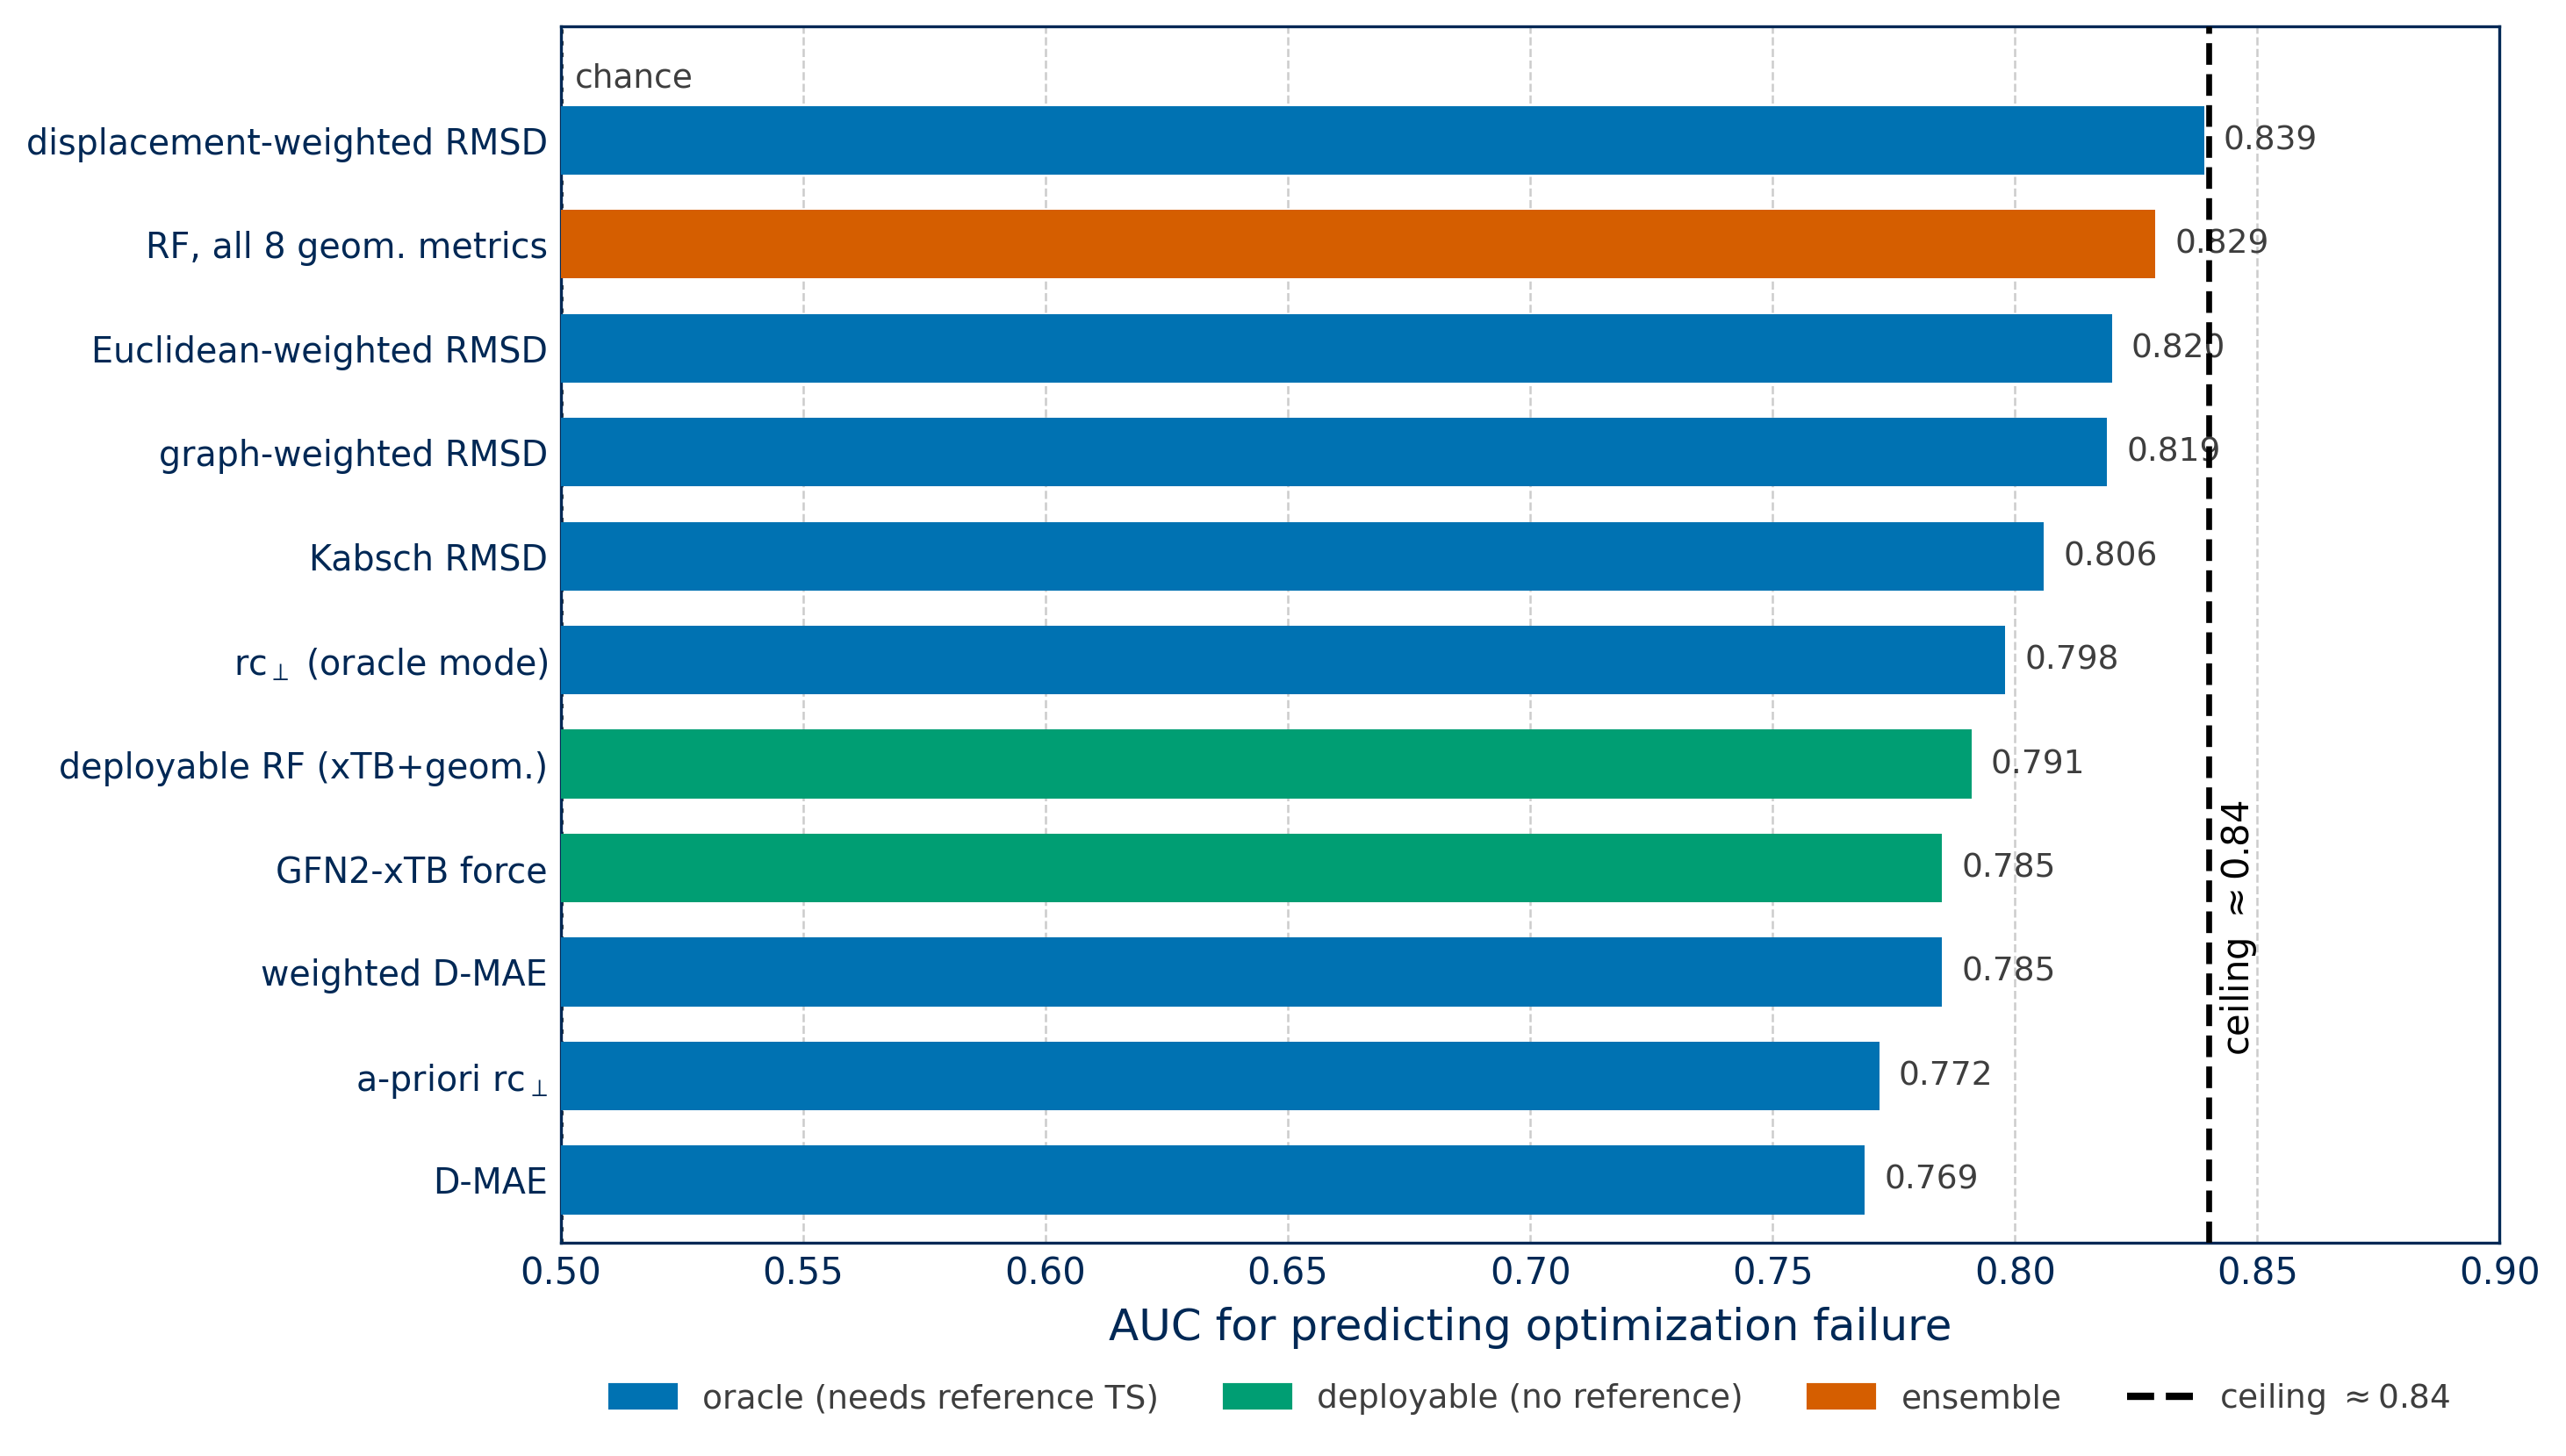
\includegraphics[width=0.82\textwidth]{../bench/plots/auc_ceiling.png}
\caption{No guess-based measure predicts optimization convergence beyond
AUC $\approx 0.84$ ($n=400$). Oracle measures (blue) require the reference
transition state; deployable descriptors (green) require only the guess and the
reactant/product; the random-forest ensemble (red) combines all eight geometric
measures. None exceeds the single displacement-weighted RMSD.}
\label{fig:ceiling}
\end{figure}

We attribute the surprising transferability of a semi-empirical force to the
r$^2$SCAN-3c optimization outcome to the breadth of the transition-state basin:
what governs convergence is not sub-\AA ngstr\"om geometric accuracy but whether
the guess lies within the basin of attraction of the saddle, a region tens of
degrees and tenths of an \AA ngstr\"om wide. GFN2-xTB, parametrised across the
periodic table for structures and reaction energetics~\cite{Bannwarth2019},
reproduces this coarse curvature and gradient structure well even where it
mis-estimates the barrier itself, so a small semi-empirical residual force is a
faithful indicator that the higher-level optimizer will fall into the same basin.
The force norm thus measures proximity to \emph{a} stationary point on a
correlated surface, which is exactly the quantity that predicts convergence.

\begin{table}[t]
\centering
\begin{tabular}{lcc}
\toprule
Measure & AUC (failure) & Needs the reference TS? \\
\midrule
Kabsch RMSD & 0.806 & yes \\
D-MAE & 0.769 & yes \\
Change-weighted D-MAE & 0.785 & yes \\
Reaction coord.\ $\perp$ error & 0.798 & yes \\
Reaction coord.\ $\parallel$ error & 0.658 & yes \\
GFN2-xTB force (guess) & 0.785 & \textbf{no} \\
Deployable random forest & 0.791 & \textbf{no} \\
\bottomrule
\end{tabular}
\caption{Every guess-quality measure saturates in the band $0.77$--$0.84$. Deployable
semi-empirical descriptors match oracle RMSD without a reference structure.}
\label{tab:auc}
\end{table}

\begin{figure}[t]
\centering
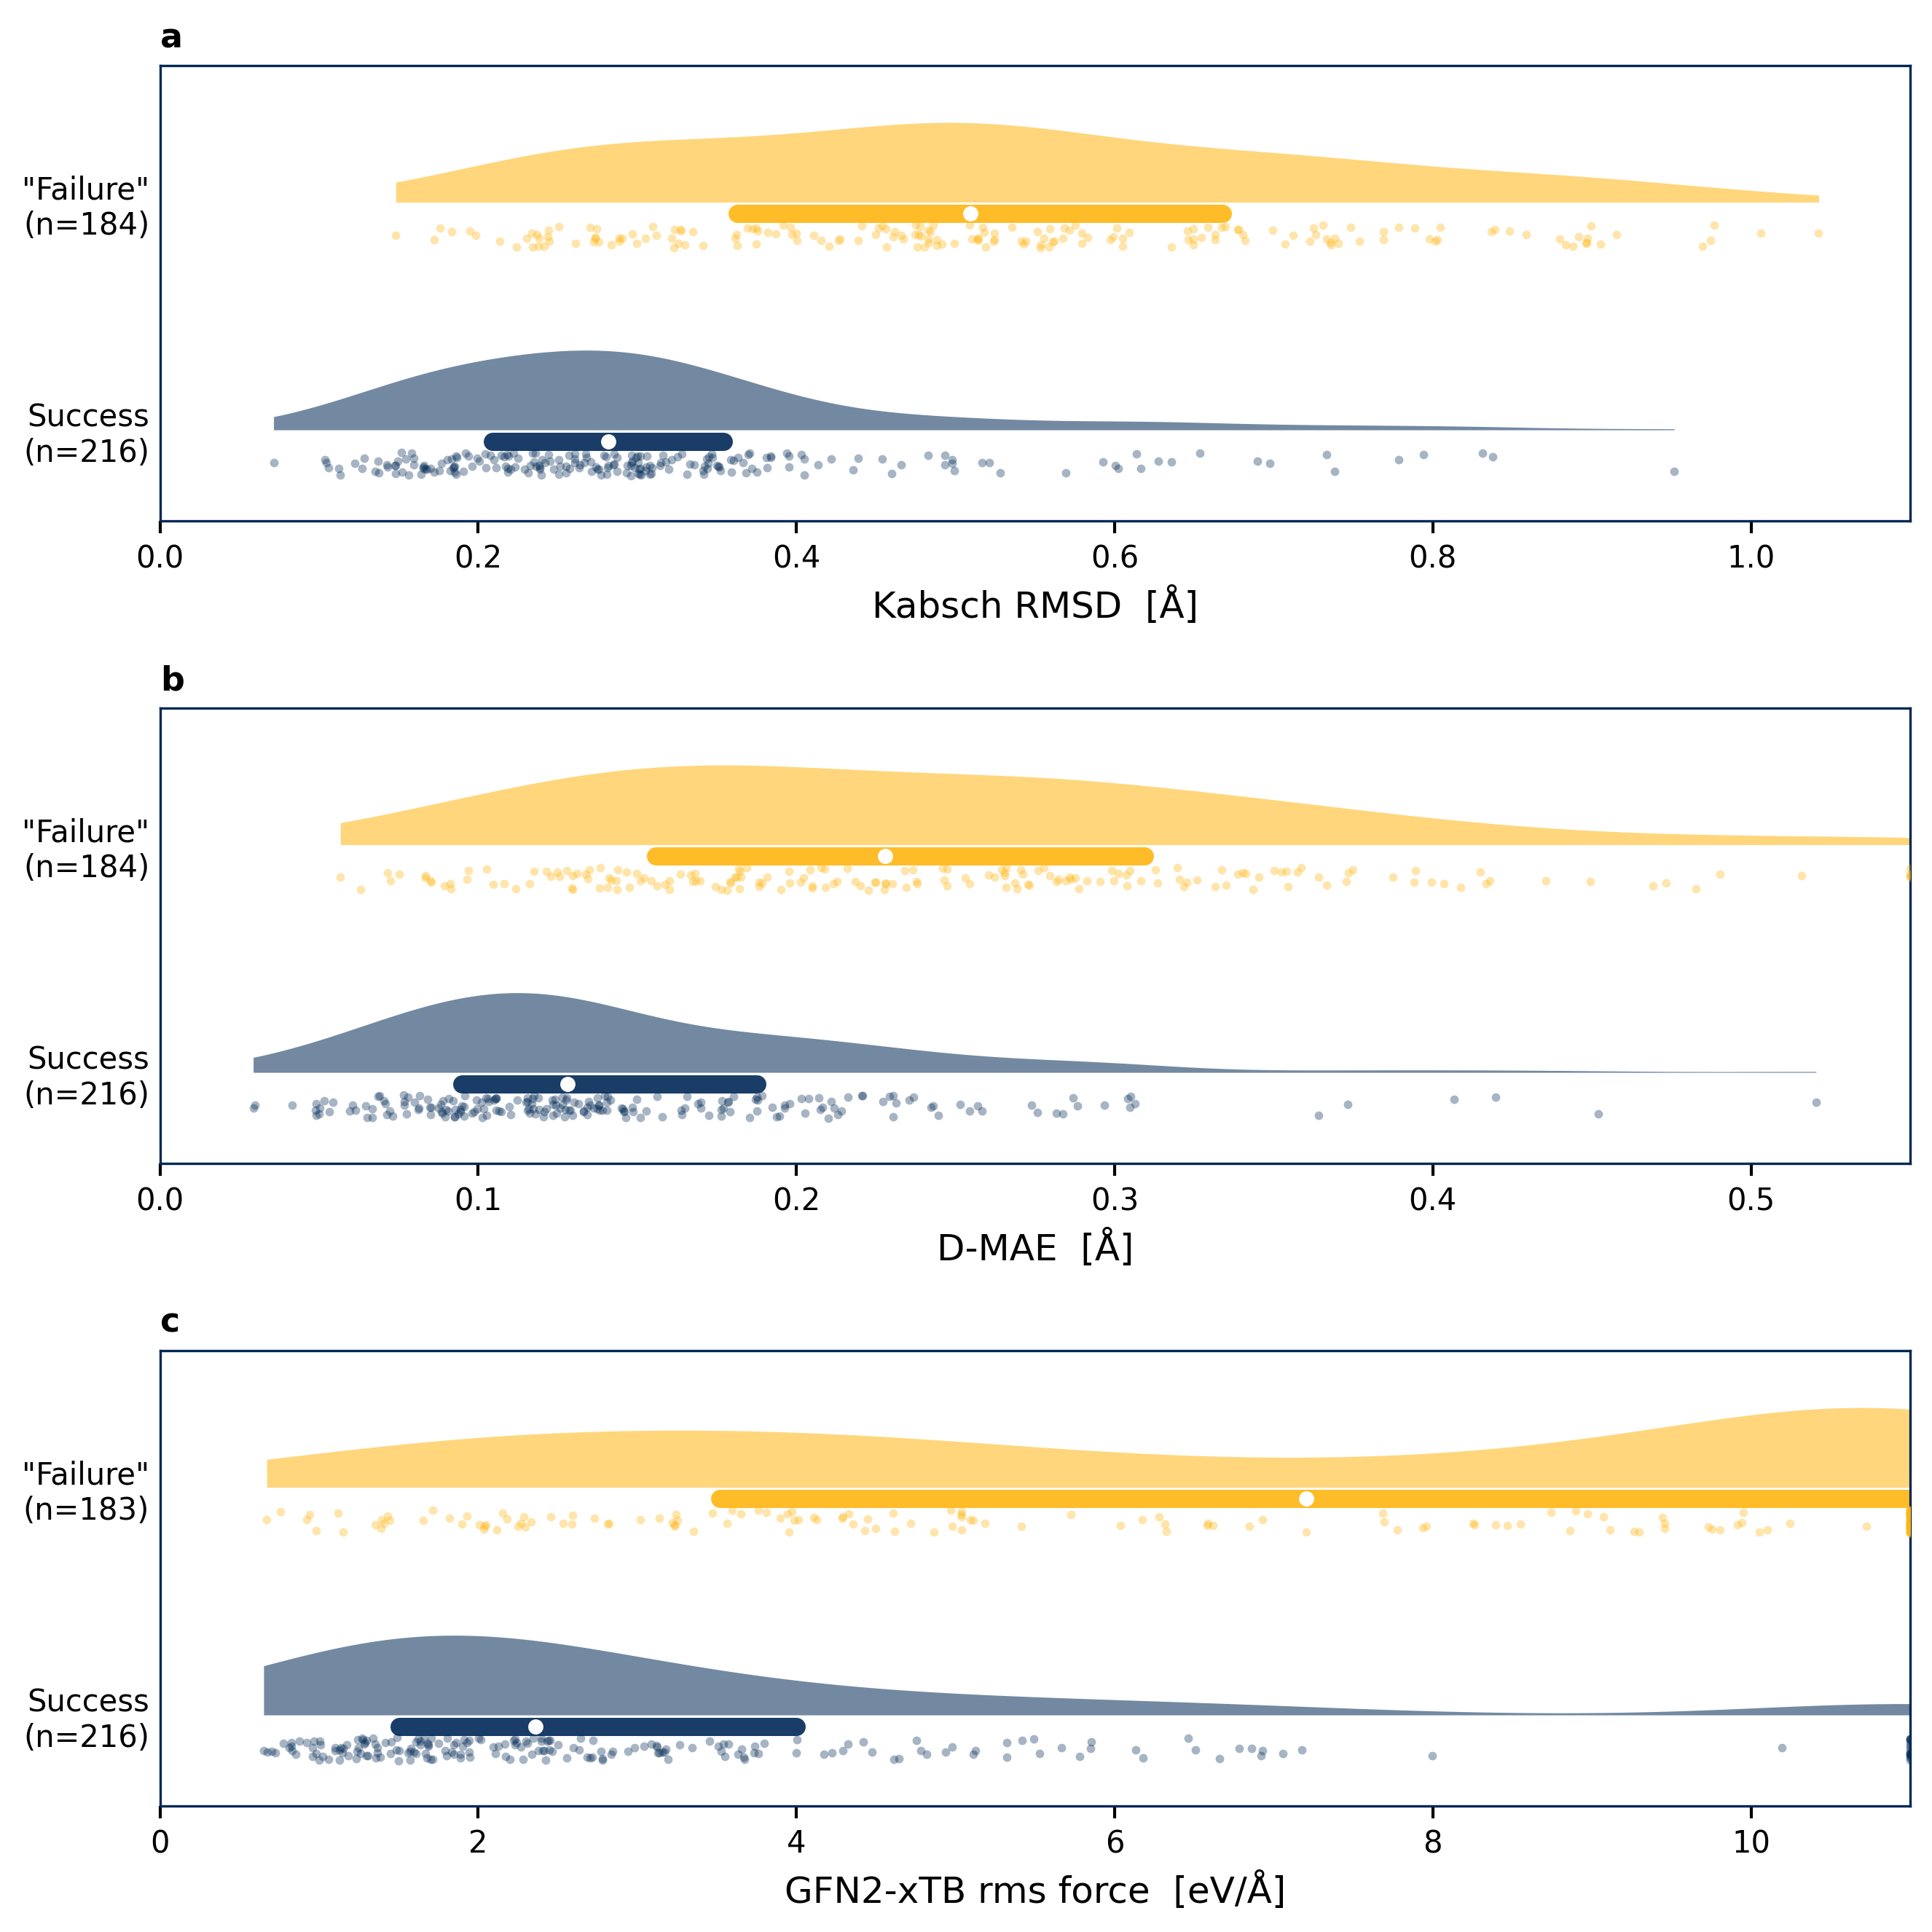
\includegraphics[width=0.9\textwidth]{../bench/plots/raincloud_by_outcome.png}
\caption{Distributions of each measure by outcome (raincloud: half-violin, box,
and per-guess points). The heavy overlap, low-metric ``failures'' and high-metric
successes, shows that no fixed RMSD cutoff separates usable from unusable guesses.}
\label{fig:dist}
\end{figure}

\subsection{A third of ``failures'' are alternative transition states}
\label{sec:alt}
Of $239$ failures, $142$ ($59\%$) do not converge, $92$ ($38\%$) converge to a
\emph{different} first-order saddle, and $5$ collapse to a minimum. For the
alternative saddles the median energy difference from the reference is $1.36$~eV,
and $77\%$ are \emph{lower} in energy; only $13\%$ lie within $0.05$~eV of the
reference (symmetry-equivalent artifacts). A third of what the metric calls
failure is therefore the optimizer locating a genuine, usually more stable,
transition state that the reference database simply does not contain. This is
consistent with reports from the generative-model literature itself: TSDiff, for
instance, was observed to sample transition states with \emph{lower} barrier
heights than the reference database~\cite{TSDiff}, which its RMSD-based evaluation
scores as deviations rather than discoveries.

The magnitude matters kinetically. A median discrepancy of $1.36$~eV
($\approx 31$~kcal\,mol$^{-1}$) in barrier height translates, through the Eyring
equation~\cite{Eyring1935}, into a factor of $\exp(\Delta E / k_\mathrm{B}T)
\approx 10^{23}$ in the predicted rate constant at $298$~K. A benchmark that
treats these saddles as errors is thus not penalizing a small geometric slip; it
is discarding transition states whose barriers differ from the reference by tens
of orders of magnitude in rate - a catastrophic outcome for any downstream
kinetic model, and precisely the regime where getting the \emph{right} saddle,
rather than one close in RMSD, is decisive.

\subsection{Convergence is a potential-energy-surface property}
Restricting to low-RMSD guesses ($<0.28$~\AA), which ``should'' converge, and
testing purely structural properties of the reactant and product, no feature
separates the $30$ failures from the $140$ successes (all AUC $0.5$--$0.6$).
Reaction-amplitude features that appear predictive over all guesses (AUC
$0.65$--$0.68$) collapse to noise once RMSD is held fixed - they predict failure
only by making the guess worse, not independently. The residual failures are
structurally indistinguishable from the successes; their cause lies in the
potential-energy surface (competing saddles, basins), not in the reaction's gross
structure.

\subsection{Cost as a graded outcome}
Convergence is binary, but its \emph{cost} --- the number of geometry-optimization
cycles --- is graded, and offers a second, more forgiving test of the metrics.
Over the guesses that do converge, the geometry measures correlate with the cycle
count only weakly to moderately (Spearman $\rho$: RMSD $0.59$, perpendicular
reaction-coordinate error $0.55$, weighted D-MAE $0.54$, D-MAE $0.51$; the cheap
GFN2-xTB force reaches $0.55$). The same ordering as for success recurs, at a
lower ceiling: a better guess is somewhat cheaper to optimize, but geometry
explains well under half the rank variance in cost. A perfect guess (the reference
TS itself) converges in $\sim 5$ cycles against $\sim 20$ for the interpolated
guesses, so the potential cost saving is large --- yet not predictable from
Cartesian similarity.

\subsection{Predictor comparison}
The bond-order predictor marginally outperforms the midpoint baseline (success
$56\%$ vs $52\%$; $20.0$ vs $21.3$ optimization cycles, paired), but the effect is
small, consistent with guess quality not being the limiting factor.

\subsection{Why the ceiling exists: a controlled displacement experiment}
\label{sec:ladder}
The results so far are correlational: guesses differ from the reference saddle in
both magnitude and character at once, so a metric's failure could reflect a poor
metric, a poor predictor, or an unforgiving surface. We separate these by
constructing displacements whose distance is fixed by design. From each reference
saddle --- first relaxed to a self-consistent GFN2-xTB saddle so that the
experiment is internally consistent --- we step a prescribed Kabsch RMSD along
four directions and repeat the saddle search: the imaginary reaction mode, the
softest real vibration, the stiffest vibration, and an isotropic Gaussian
direction. Rigid-body components are projected out and the step length is solved
numerically, so every trial sits at the requested distance to better than
$10^{-3}$~\AA; the achieved distance is recorded for every trial and audited.
A trial ``returns'' if the search converges to the same saddle within $0.3$~\AA.

\begin{figure}[t]
\centering
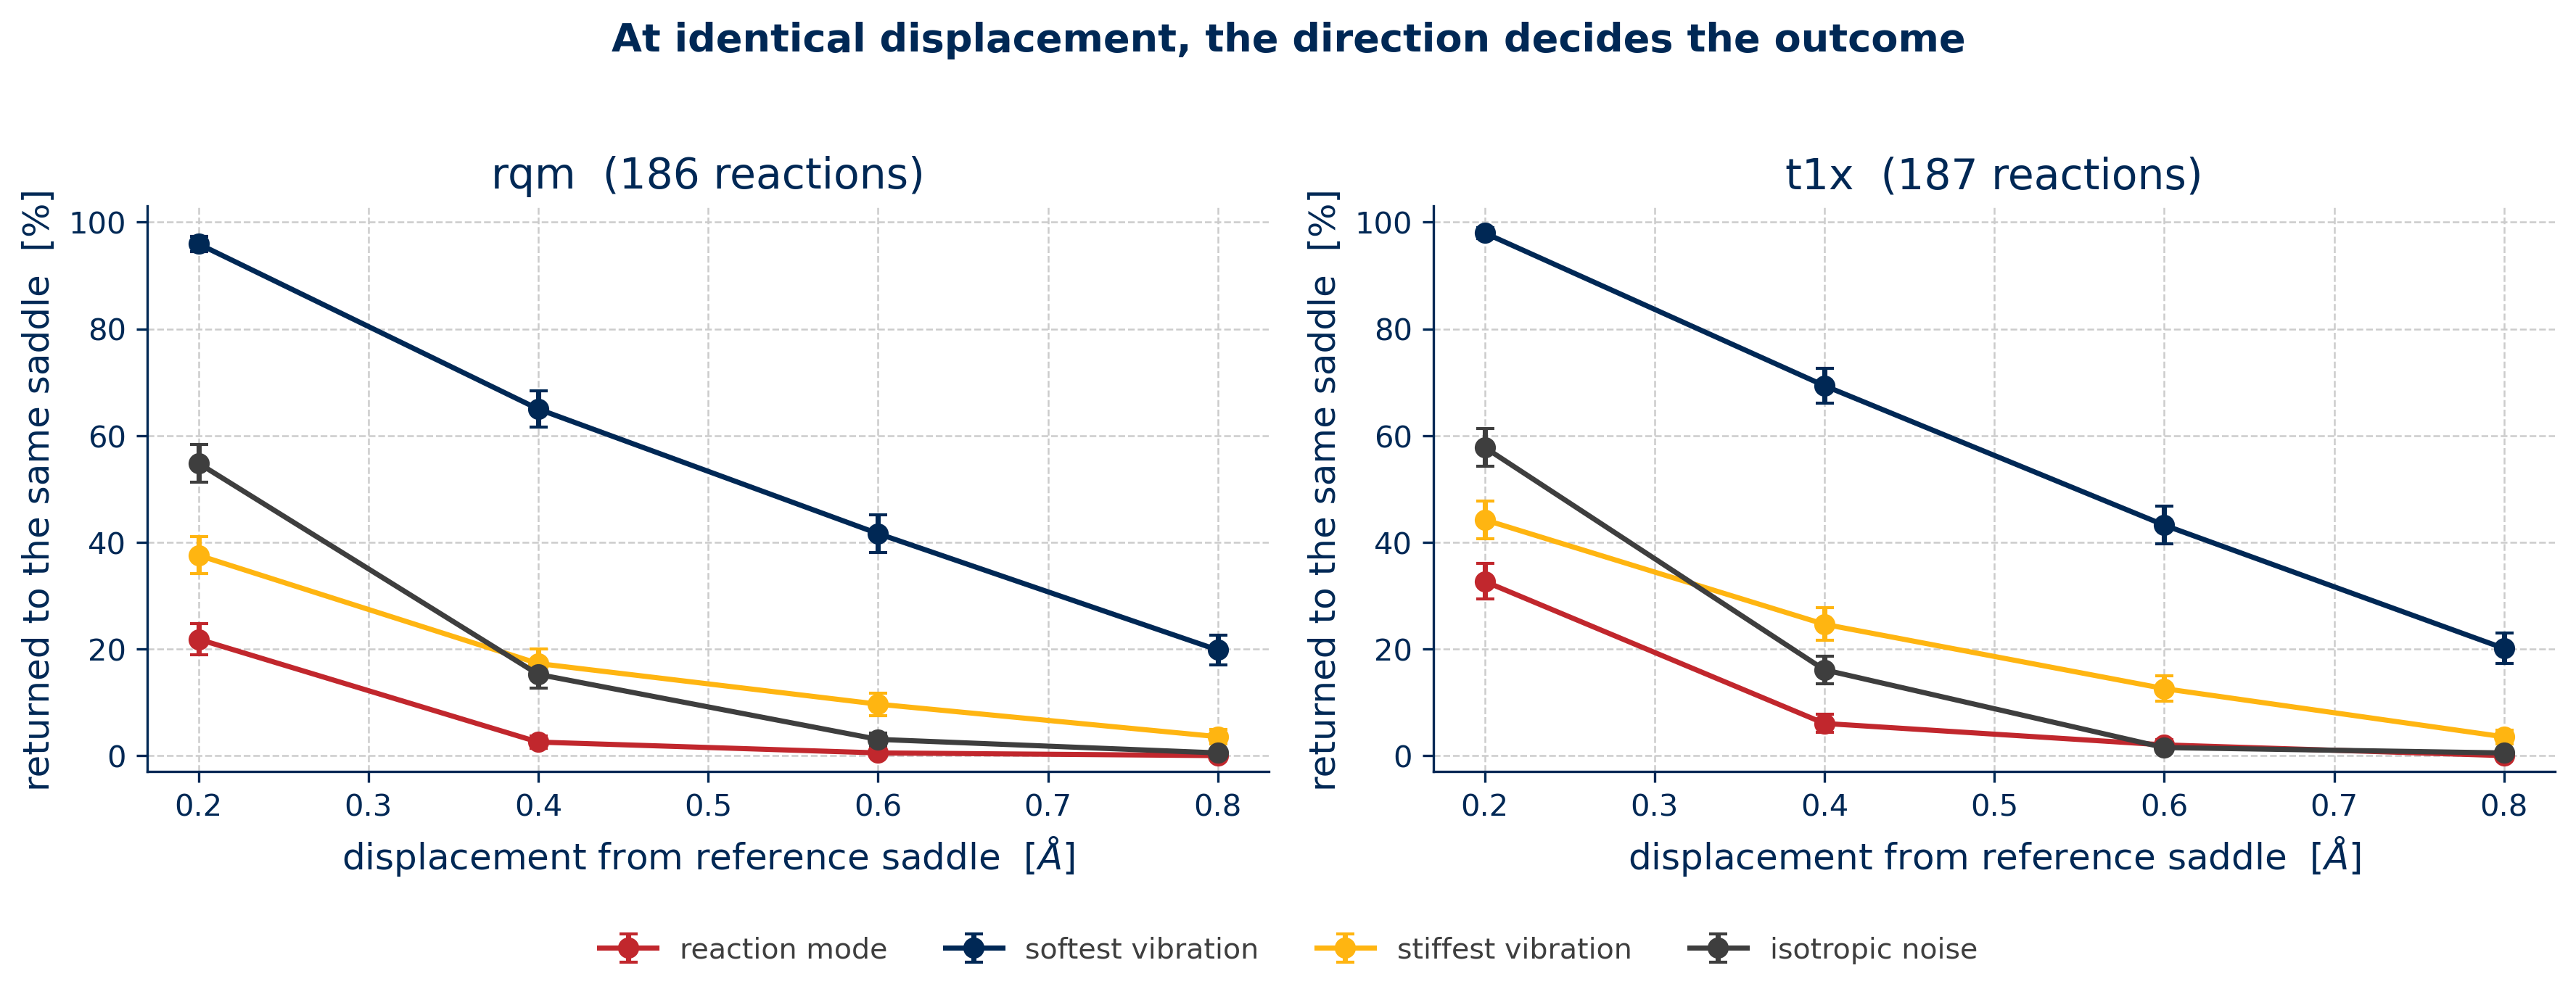
\includegraphics[width=\textwidth]{../bench/plots/ladder.png}
\caption{Controlled displacement from the reference saddle ($187$ and $186$
reactions, ${\sim}3\,200$ trials per database). Every point at a given abscissa
sits at an \emph{identical} distance from the saddle --- verified to
$10^{-3}$~\AA\ for every trial --- so the vertical spread is due to direction
alone. Error bars are binomial standard errors.}
\label{fig:ladder}
\end{figure}

At a fixed displacement of $0.20$~\AA, the return rate ranges from $33\%$ along
the reaction mode to $98\%$ along the softest vibration on Transition1x, and from
$22\%$ to $96\%$ on Reaction-QM (Figure~\ref{fig:ladder}); direction-independence
is rejected overwhelmingly at every displacement in both databases ($\chi^2$ on
$3$ degrees of freedom, $p<10^{-16}$ throughout, reaching $p=6\times10^{-36}$).
The ordering is physically sensible and identical across the two databases: the
reaction mode is the unstable direction and leaves the basin fastest, while the
softest vibration is the most forgiving. \emph{Cartesian distance therefore
cannot determine the outcome, because outcomes spanning $33\%$ to $98\%$ share
the same distance.}

Controlling direction as well recovers part, but only part, of the lost
discrimination. Pooled over directions, the area under the curve for displacement
predicting failure to return is $0.770$ (Transition1x) and $0.757$
(Reaction-QM); restricted to a single direction it rises to $0.828$ and $0.822$.
Direction-blindness thus costs roughly $0.06$ in area under the curve --- a real
but modest penalty, and far from the whole gap to a perfect predictor. The
residue is the point: even with the distance controlled to $10^{-3}$~\AA, the
direction held fixed, and the reference saddle identical, displacement predicts
return only at AUC $\approx 0.83$. That is essentially the value reached by the
best purely geometric measure on real predictions (displacement-weighted RMSD,
$0.839$, Table~\ref{tab:weights}).

Because these displacements are drawn from a small set of prescribed lengths,
almost every pair of trials is tied in distance; areas under the curve are
therefore computed with mid-ranks, without which ties are broken arbitrarily and
the statistic becomes meaningless.

The experiment was repeated at the working level of theory to confirm that it is
not an artifact of the semi-empirical surface: $320$ additional r$^2$SCAN-3c
saddle optimizations on $40$ Transition1x reactions, with the displacement
directions taken from the reference DFT Hessians rather than recomputed. The
direction effect reproduces ($98\%$ return along the softest vibration against
$28\%$ along the reaction mode at $0.20$~\AA; $p=3\times10^{-8}$ and
$8\times10^{-14}$ at the two displacements). Compared like for like --- the same
$40$ reactions and the same two displacements --- the two levels of theory agree
to within $0.01$ in area under the curve (pooled $0.651$ at r$^2$SCAN-3c against
$0.665$ at GFN2-xTB; within-direction $0.711$ against $0.722$), so the
semi-empirical surface is a faithful proxy here and the larger xTB sample can
carry the statistical weight. The lower absolute values in this comparison are
themselves an instance of the range effect of Section~\ref{sec:rqm}: restricting
the same xTB data from four displacements to two moves the within-direction area
from $0.828$ to $0.702$.

Two independent routes therefore arrive at the same number. This is the
mechanism. The ceiling is not an artifact of metric design, nor merely of RMSD's
blindness to direction, nor of noise in the predictors: it survives an experiment
in which all three are eliminated or controlled by construction. What remains is
irreducible variation between reactions in how large a basin their saddle
possesses --- a property of the potential energy surface that no measurement of
the guess geometry can access. Metrics saturate near $0.83$ because that is where
the information in a guess geometry runs out, and the best of them already
operates at that limit.

A corollary bears on how synthetic guesses should be built. Isotropic Gaussian
noise, the natural way to manufacture guesses of a prescribed quality, does not
behave like a typical direction: it tracks the \emph{reaction mode} arm, the
harshest of the four. Perturbing a reference structure isotropically therefore
understates the success rate a real predictor would achieve at the same nominal
deviation, and is not a neutral surrogate for predictor error.

\subsection{Generalization to a second, harder database}
\label{sec:rqm}
All results above derive from a single database of small first-row organic
reactions. To test whether they are an artifact of that chemistry, we repeated the
entire protocol on $200$ unimolecular reactions drawn from the density-functional
subset of Reaction-QM~\cite{ReactionQM2026}, which extends to second- and
third-row elements (Si, P, S, Cl) and larger systems. Reference saddles behave as
before ($197/200$ converged, all with exactly one imaginary frequency), so
the comparison is not confounded by a poor reference.

Three things change, and one does not (Figure~\ref{fig:generalization}). First, the predictors degrade sharply
out of distribution: the median guess deviation rises from $0.35$~\AA\ to
$1.02$~\AA, and only $2$ of $400$ guesses fall below $0.3$~\AA\ (against $155$ of
$400$ on Transition1x). Second, downstream success collapses from $54\%$ to
$6\%$, with convergence falling from $73\%$ to $34\%$ and the median cost of a
converged optimization rising from ${\sim}20$ to ${\sim}32$ cycles. Third, the
fraction of converged guesses that reach an alternative saddle rather than the
reference one \emph{grows}, from $19\%$ to $26\%$: as reactions become more
complex, the reference transition state accounts for a smaller share of the
accessible saddles, reinforcing Section~\ref{sec:irc}.

\begin{figure}[t]
\centering
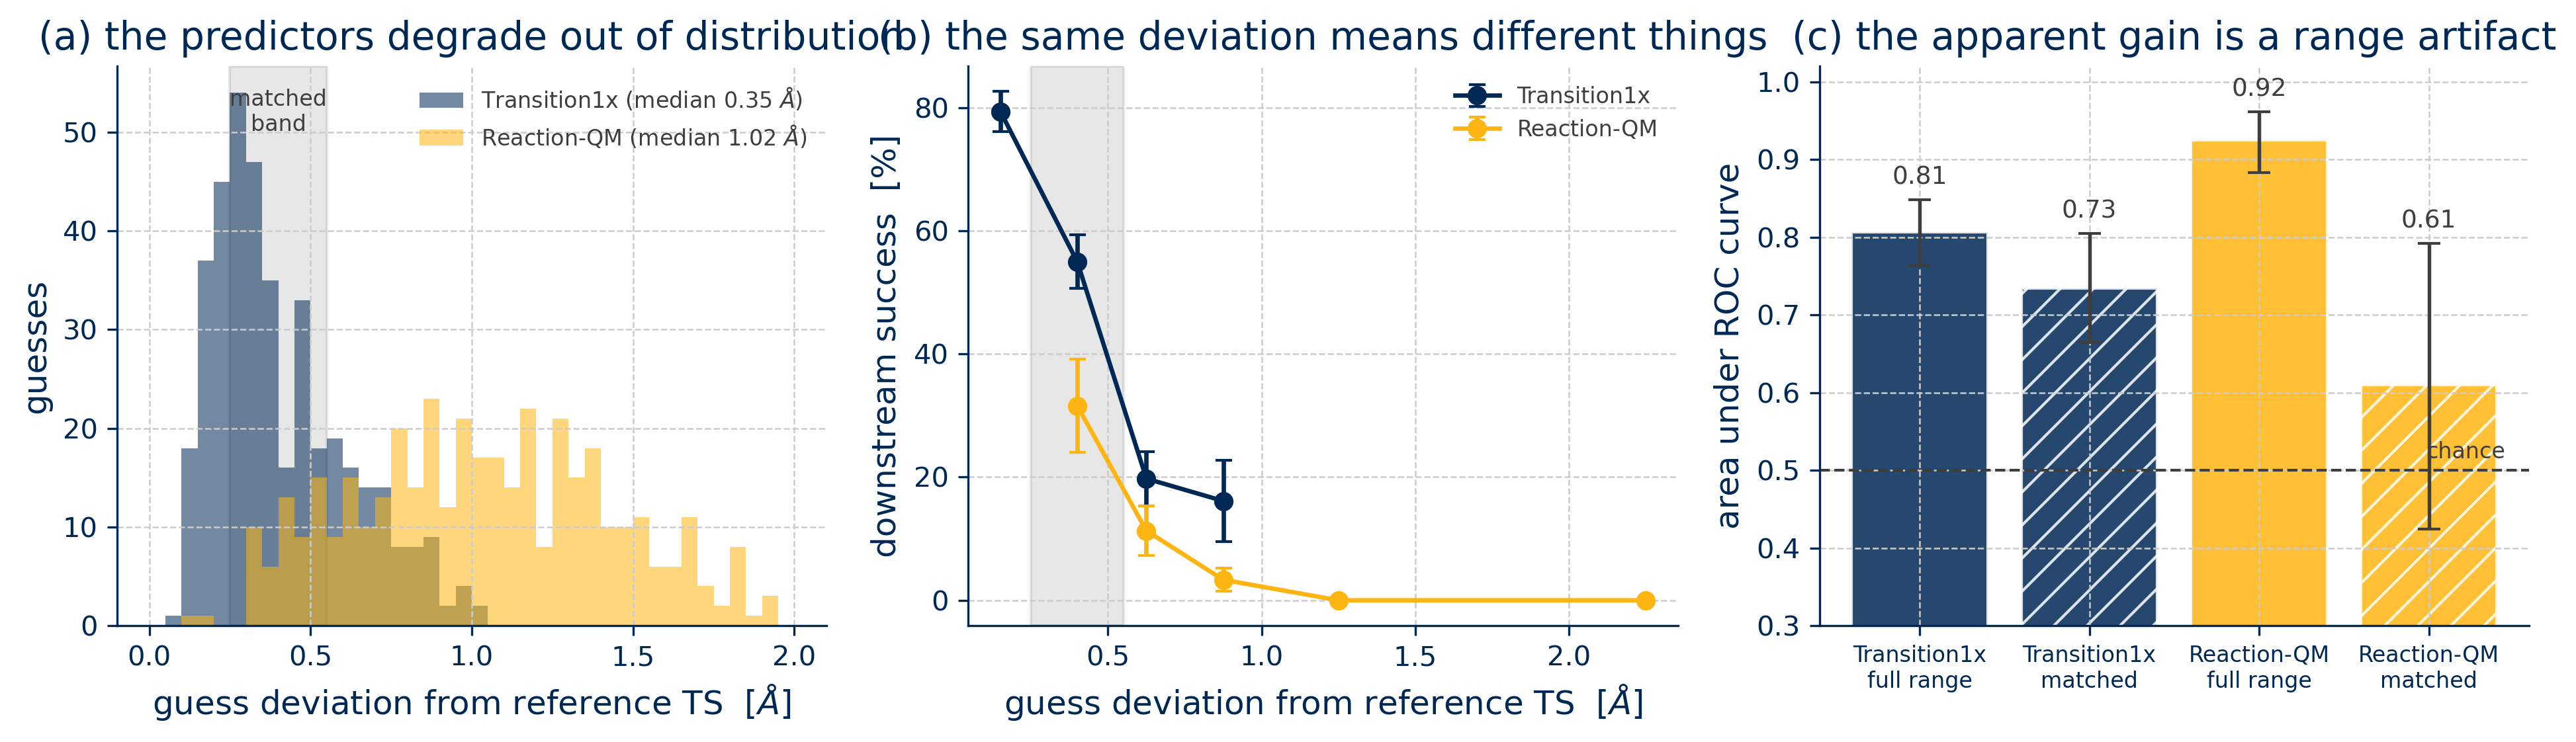
\includegraphics[width=\textwidth]{../bench/plots/generalisation.png}
\caption{Generalization to Reaction-QM. (a) The predictors degrade sharply out of
distribution; the shaded band is the Transition1x interquartile range of guess
deviation, used to match the two datasets. (b) Downstream success against guess
deviation: at every matched deviation Reaction-QM succeeds less often, so a
threshold calibrated on one database does not transfer to the other. (c) The
apparent improvement in discrimination on Reaction-QM ($0.92$) is an artifact of
its much wider deviation range; restricted to the matched band it falls to
$0.61$, statistically indistinguishable from both the Transition1x value and from
chance. Error bars are binomial standard errors in (b) and $95\%$ bootstrap
confidence intervals in (c).}
\label{fig:generalization}
\end{figure}

What does not change is the central negative result. Taken over the full range,
the area under the receiver-operating-characteristic curve for the deviation
measure appears to \emph{improve} to $0.92$, which would suggest the ceiling of
Section~\ref{sec:ceiling} had been broken. It has not. That figure is an artifact
of range: discrimination is trivially easier when the guesses span a wide quality
range ($0.74$--$1.33$~\AA\ interquartile) than a narrow one
($0.25$--$0.54$~\AA). Restricting the Reaction-QM guesses to the Transition1x
interquartile range removes the advantage entirely --- the area under the curve
falls to $0.61$ ($95\%$ bootstrap confidence interval $0.42$--$0.80$, $n=53$),
statistically indistinguishable from both the Transition1x value of $0.73$
($0.66$--$0.81$) and from chance. Geometric similarity to the reference
transition state is therefore no more predictive on a harder and chemically
broader database than on the one the conclusion was drawn from; if anything the
mapping from deviation to outcome is itself database-dependent, so a threshold
calibrated on one dataset does not transfer to another.

The one result that does replicate is the predictor ordering: the bond-order
predictor again edges out the midpoint baseline ($7\%$ vs $5\%$ success), the
same direction and the same negligible magnitude as before.

\subsection{The same ceiling constrains a state-of-the-art generative model}
\label{sec:generative}
The predictors studied so far are deliberately simple. A natural objection is
that the ceiling is a property of weak, interpolation-based guesses and would
lift for a modern machine-learned generator. We therefore repeated the analysis
with RitS~\cite{RitS}, a flow-matching transition-state generator that takes the
reactant and product geometries and emits a predicted saddle. We use the authors'
released checkpoint, which is not trained on Transition1x, so our evaluation
carries no train--test leakage. Two limits of the tool bound its coverage and are
reported rather than hidden: it supports only the elements C, H, N, O, S, F, P
(removing $96$ of the $200$ Reaction-QM reactions), and its bond perception from
Cartesian input fails outright on $16$ of $200$ Transition1x and $7$ of the
remaining $104$ Reaction-QM reactions, leaving $184$ and $97$ reactions.

The first observation is that the generator is \emph{stochastic}: each call draws
an independent sample, and the ten draws for a single reaction span a median
range of $0.67$~\AA\ on Transition1x (Figure~\ref{fig:generative}a) --- wider than
the entire spread between the methods compared in the rest of this paper. This
makes the choice of what to report decisive. The single draw a user actually
obtains has a median deviation of $0.82$~\AA\ (Transition1x) and $1.08$~\AA\
(Reaction-QM), no better than the linear-interpolation baseline. The
\emph{best} of ten draws, selected by proximity to the reference saddle, has a
median deviation of $0.37$ and $0.73$~\AA\ --- a two- to threefold improvement,
and the number a best-of-$N$ benchmark would report.

That best-of-$N$ number is an oracle. Selecting the closest sample requires the
reference transition state, which is exactly the unknown the model exists to
predict. The gap it opens is not academic: optimized at r$^2$SCAN-3c under our
success criterion, the deployable single draw reaches the reference saddle for
$16\%$ (Transition1x) and $4\%$ (Reaction-QM) of reactions, while the oracle
best-of-ten reaches it for $44\%$ and $23\%$ (Figure~\ref{fig:generative}c;
McNemar $p<10^{-3}$ on both, discordant pairs $54$ vs $2$ and $18$ vs $0$).
Oracle selection roughly triples the success rate --- a gain entirely unavailable
at prediction time.

The obvious question is whether a \emph{reference-free} score can recover it. We
tried three: the consensus (medoid) sample, which requires no electronic
structure; the lowest GFN2-xTB force, which is the deployable descriptor this
paper recommends elsewhere; and the lowest GFN2-xTB energy. None works. Across
both databases the sample each selects sits at a mean rank of $4.5$--$5.7$ among
the ten (Figure~\ref{fig:generative}b), against a chance expectation of $5.5$ and
the oracle's $1.0$; the consensus sample is marginally better than chance and the
energy and force selectors are not. The near-threefold best-of-$N$ advantage is
therefore real but structurally inaccessible: it lives in knowing which sample is
closest to an answer one does not have, and no cheap proxy stands in for that
knowledge. The information ceiling of Section~\ref{sec:ceiling} thus reappears for
a modern generator in a sharper form --- as a selection problem --- and it cautions
that best-of-$N$ scores in the generative-TS literature overstate deployable
performance by roughly a factor of three.

\begin{figure}[t]
\centering
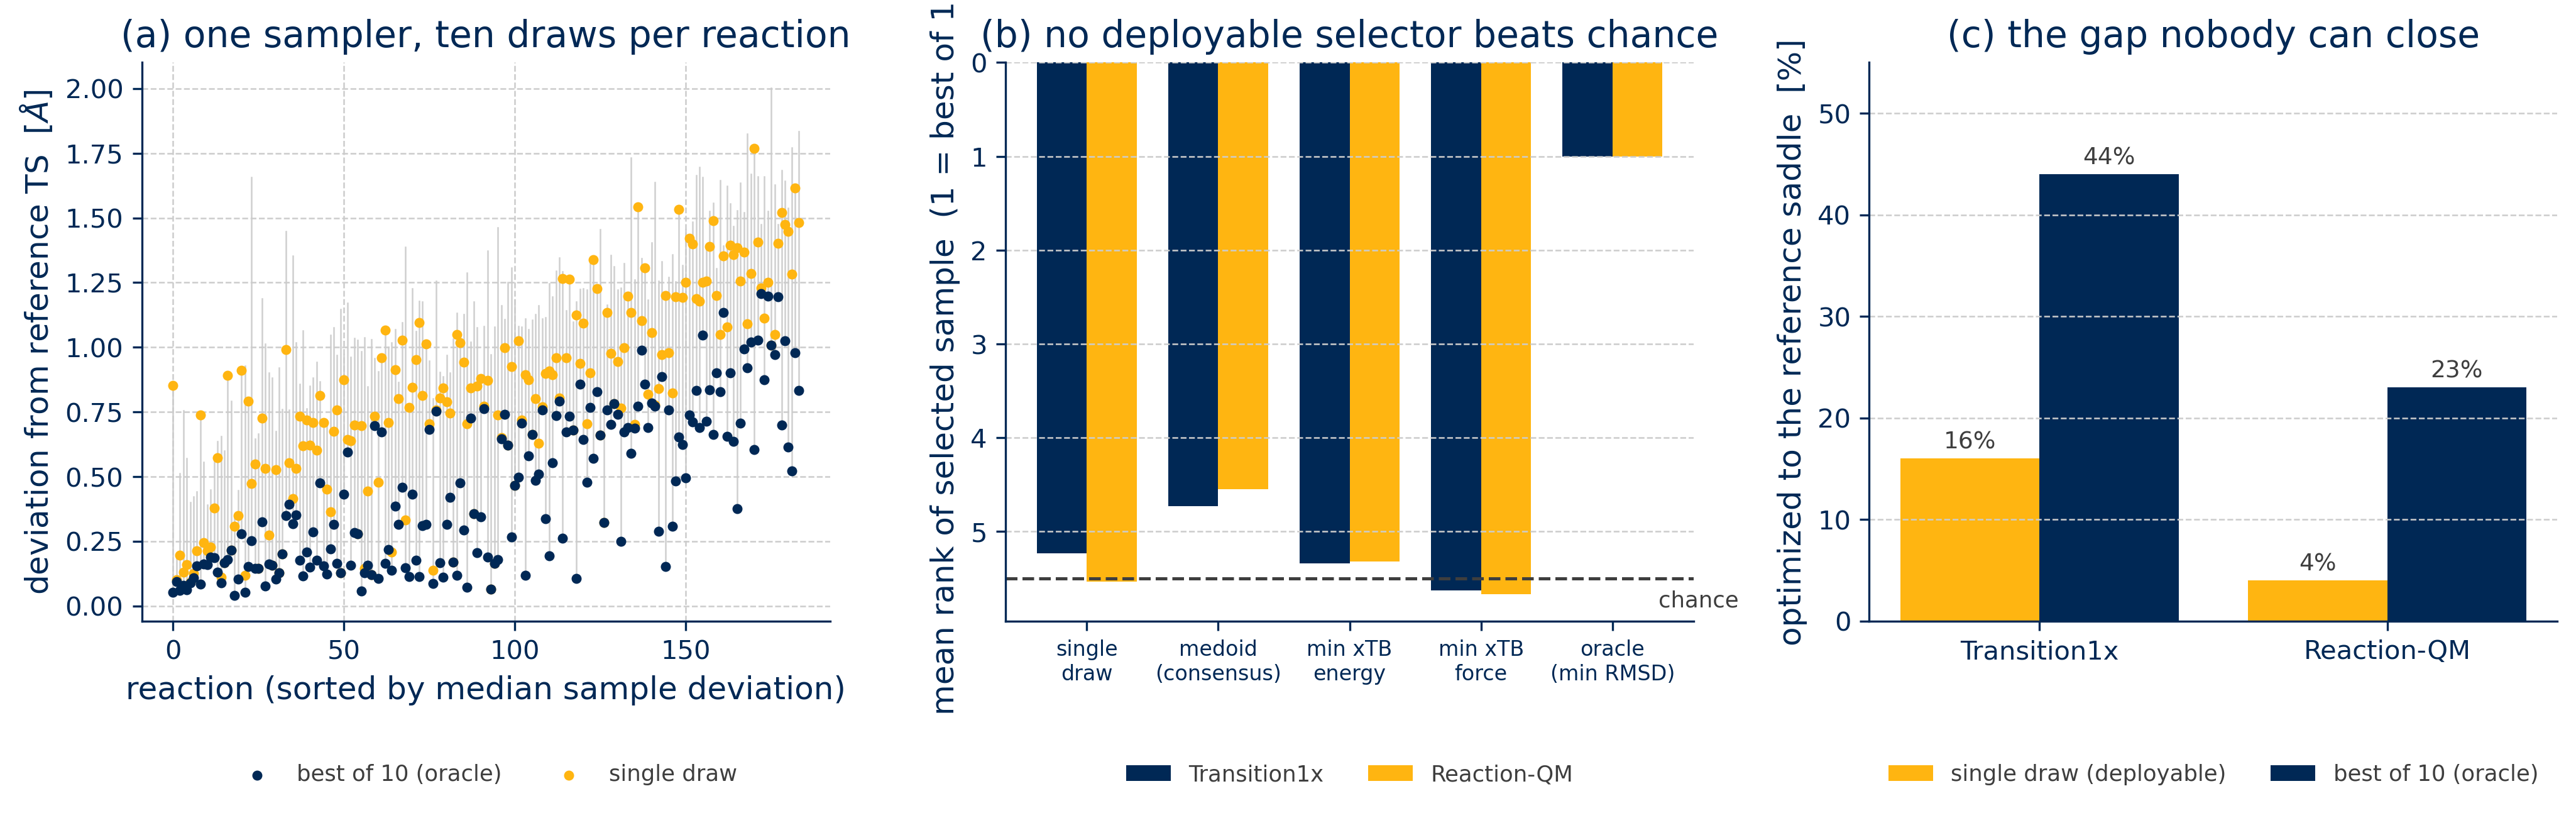
\includegraphics[width=\textwidth]{../bench/plots/generative.png}
\caption{A state-of-the-art generator under the same lens. (a) RitS is
stochastic: for each Transition1x reaction (sorted by median), ten draws span a
wide range; the oracle best (blue) sits far below the single draw (orange).
(b) Mean rank of the sample chosen by each reference-free selector, out of ten
($1=$ best); every deployable selector lands near the chance line, only the
oracle (min RMSD to the reference) reaches $1$. (c) Optimized at r$^2$SCAN-3c, the
oracle best-of-ten roughly triples the deployable single-draw success on both
databases --- a gap no reference-free selector closes.}
\label{fig:generative}
\end{figure}

\subsection{The nature of the alternative saddles is not reliably determinable}
\label{sec:irc}
We attempted to classify each alternative saddle by computing its intrinsic
reaction coordinate (IRC) at r$^2$SCAN-3c and identifying the two endpoints
(after a short GFN2-xTB relaxation of the frequently truncated IRC endpoints).
Reference-transition-state controls, whose IRCs must connect their reactant and
product, validated the endpoint extraction ($6/6$). Symmetry-equivalent artifacts
(energy within $0.05$~eV of the reference) account for $\sim 13\%$ of the
alternative saddles and were removed.

However, assigning the remaining endpoints to a chemical species proved
\emph{not robust}. Four reasonable identity criteria - covalent adjacency
graph, InChI, RMG-Py graph isomorphism (as used by the Automated Rate Calculator,
ARC~\cite{ARC}), and canonical SMILES - returned between
$6\%$ and $91\%$ ``same reaction'' on the identical set of endpoints. Manual
inspection identified three specific algorithmic blind spots, all aggravated by
the open-shell character of many Transition1x species. First, \emph{radical-center
and multiplicity assignment} is not consistent across two geometries of the same
molecule: perception routines placed unpaired electrons on different atoms and
returned different multiplicities for a species and its own relaxed copy. Second,
\emph{resonance-structure selection} is arbitrary - a delocalised radical is
represented by one of several equivalent Kekul\'e/resonance forms, and graph
isomorphism then declares two forms of the same species distinct. Third,
\emph{path directionality} is lost: an IRC endpoint may relax to a conformer or
tautomer of the reactant/product that the reference minimum does not match, and
the two IRC branches occasionally invert, so reactant and product labels swap.
The net effect is that a single species is repeatedly split into spurious
``intermediates'' (many carried a SMILES string identical to the product yet were
flagged distinct; Figure~\ref{fig:blind}). We therefore \emph{cannot} state with
confidence whether the
alternative saddles are concerted alternatives of the same reaction, genuine
stepwise elementary steps, or saddles of different reactions. This is itself a
finding: for open-shell reaction networks, even the seemingly simple question
``did the guess find the intended reaction?'' is not answerable by current
automated structure perception, and a robust, perception-independent connectivity
criterion is an open problem. What we can state solidly, the foregoing
notwithstanding, rests on energetics alone: the alternative saddles exist, are
usually lower in energy, and are penalized by a reference-matching metric.

\begin{figure}[t]
\centering
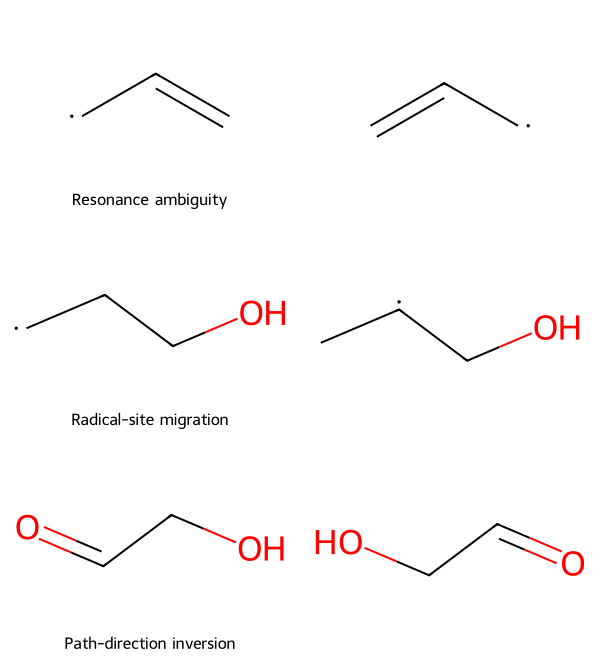
\includegraphics[width=0.85\textwidth]{../bench/plots/blind_spots.png}
\caption{Three algorithmic blind spots that make automated species perception
inconsistent for open-shell IRC endpoints, each illustrated by a pair that is
chemically one species yet is repeatedly assigned two identities. \emph{Left/right
within each row}: (top) resonance ambiguity, a delocalised radical represented by
two equivalent forms; (middle) radical-site migration, the unpaired electron
placed on a different atom for two geometries of the same molecule; (bottom)
path-direction inversion, an IRC whose two branches relax to reactant/product
labels that swap. These failures underlie the $6\%$--$91\%$ spread across identity
criteria in Section~\ref{sec:irc}.}
\label{fig:blind}
\end{figure}

\section{Discussion}

\paragraph{Cartesian distance is a flawed proxy for surface topology.}
RMSD and D-MAE measure proximity to \emph{one} recorded saddle, whereas what a
practitioner needs is that the guess lie in the basin of attraction of \emph{a}
valid saddle connecting reactant and product - a topological property. The two
notions coincide only when the reference is the unique relevant saddle, which we
find fails roughly a third of the time.

\paragraph{Reference databases are energetically skewed.}
Interpolation guesses routinely optimize to lower-energy saddles ($77\%$ of the
alternative-saddle cases) absent from Transition1x. A geometrically ``wrong''
prediction frequently reaches a more stable transition state. Benchmarking
against a single reference rewards a model for reproducing the database's
particular saddle choice rather than for locating a valid, possibly better,
transition state - even though (Section~\ref{sec:irc}) we cannot robustly
determine, for these open-shell endpoints, whether each lower saddle belongs to
the same reaction, a stepwise variant, or a different one.

\paragraph{Local optimizers are Hessian-blind.}
A quasi-Newton saddle-point optimizer only ever sees the local Hessian; from a
given guess it walks to whichever saddle the local curvature indicates, which need
not be the closest in RMSD nor the reference. This is why no function of the guess
geometry predicts convergence beyond AUC $\approx 0.84$: the outcome is fixed by
the surface, not the guess. Our controlled-displacement experiment makes this
concrete --- direction at fixed distance swings the outcome from $33\%$ to $98\%$,
and even the direction-controlled ceiling matches the best real metric --- so the
saturation is an information limit, not a modeling artifact.

\paragraph{For generative models the ceiling becomes a selection problem.}
A stochastic generator can place a good saddle among its samples far more often
than any single draw suggests: for RitS the oracle best of ten roughly triples
the deployable success rate. But choosing that sample requires the reference, and
none of the reference-free scores we tried --- consensus, xTB force, xTB energy ---
selects better than chance. Best-of-$N$ evaluation therefore measures the wrong
quantity: it credits a model for a sample it cannot identify without the answer,
and overstates deployable performance by about threefold. The honest figure is
the expected quality of a \emph{single} draw, or of a draw selected by a genuinely
reference-free rule.

\paragraph{Toward better objectives.}
The community should (i)~report convergence rate and IRC connectivity rather than
RMSD/D-MAE; (ii)~score against \emph{any} valid reactant$\rightarrow$product
saddle rather than a single reference; (iii)~for stochastic generators, report
single-draw or reference-free-selected quality rather than oracle best-of-$N$; and
(iv)~explore topological or energy-derivative-free training objectives (for
instance a force-norm or saddle-character penalty) that reward residence in a
saddle basin over proximity to a particular geometry. For a cheap convergence
proxy at scale, a GFN2-xTB force descriptor on the guess is about as informative
as oracle RMSD and needs no reference structure.

\section{Conclusion}
Geometric similarity to a reference transition state does not predict whether a
predicted geometry is useful: every geometry metric saturates in a narrow band
below AUC $0.84$,
and a large share of apparent failures are lower-energy saddles the reference
database omits and the metric penalizes. A controlled experiment locates the
cause. At a fixed distance from the saddle the outcome varies from $33\%$ to
$98\%$ depending only on the direction of displacement, so distance cannot
determine convergence; yet once direction is \emph{also} controlled the ceiling
persists at AUC $\approx 0.83$, and the effect reproduces at r$^2$SCAN-3c. The
saturation is therefore not a deficiency of
any particular metric but a limit on what guess geometry can express: reactions
differ irreducibly in the size of the basin around their saddle. This holds on a second, chemically
broader database: once the comparison is matched for guess quality, geometric
similarity is no more predictive there than on the database the conclusion was
drawn from, and the mapping from deviation to outcome does not transfer between
the two. The same limit constrains a state-of-the-art generative model: its
oracle best-of-$N$ score, roughly triple its deployable single-draw success,
cannot be recovered by any reference-free selection rule, so reported best-of-$N$
figures do not reflect what a user obtains. Transition-state prediction should be
benchmarked by surface behavior - convergence, and where determinable,
connectivity - not by Cartesian distance, and generative models by the quality of
a single or reference-free-selected draw rather than an oracle best-of-$N$. That
determining connectivity is itself hard for open-shell reaction networks only
underscores that geometric distance is the wrong yardstick.

\section*{Data and code}
\begin{sloppypar}
Analysis scripts (\texttt{bench/}) and reduced datasets (\texttt{server/}) are
provided; DFT jobs were generated by \texttt{make\_orca\_jobs.py},
\texttt{make\_orca\_ladder.py} (controlled displacement) and
\texttt{make\_orca\_rits.py} (generative guesses), and reduced on the cluster to
compact JSON by \texttt{reduce\_batch.py} / \texttt{reduce\_ladder.py}. RitS
guesses and reference-free selectors are produced by \texttt{run\_rits.py} and
\texttt{rits\_selectors.py}.
\end{sloppypar}

\bibliographystyle{unsrt}
\bibliography{refs}

\end{document}
